\chapter{Analýza a pravidla hry}

\section{Pravidla}
Pravidla hry TickoaTTwo jako první určil \textcite{jenkins22}.

Stejně jako tradiční piškvorky, hra TickoaTTwo se hraje na hrací ploše o
velikosti 3x3. Hrací plocha má dle původní definice hry specifický vzhled jako
na obrázku \ref{fig:empty-board}.

\begin{figure}[h]
    \centering
    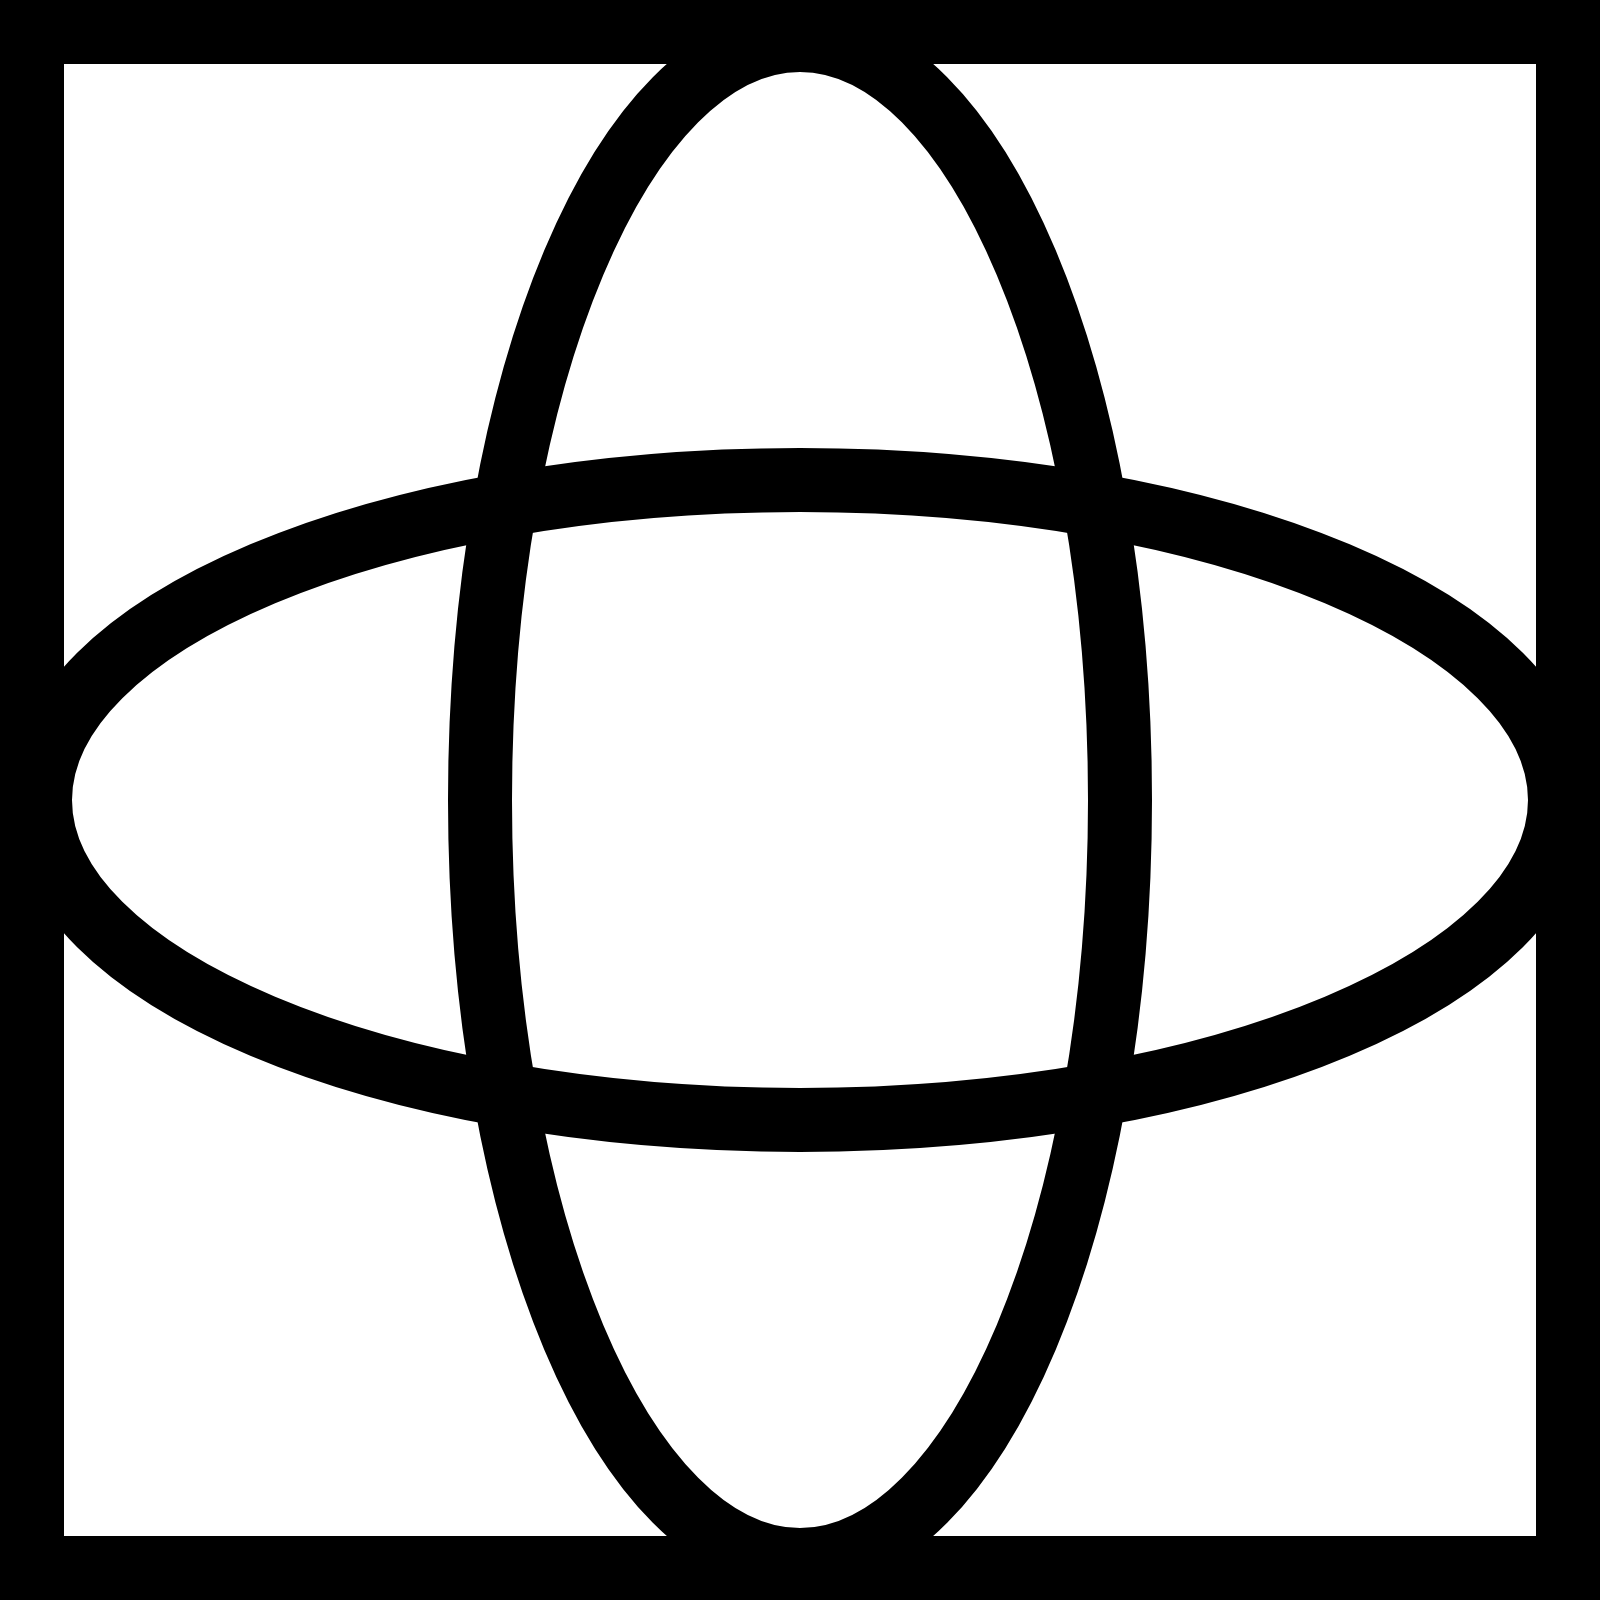
\includegraphics[width=300px]{img/empty-board.png}
    \caption{Prázdná herní plocha}
    \label{fig:empty-board}
\end{figure}

Stejně jako tradiční piškvorky, hru TickoaTTwo proti sobě hrají dva hráči,
kteří se střídají v tazích. Jeden hráč na políčka v hrací ploše kreslí svislé
čáry, druhý hráč vodorovné čáry. Na každé políčko může daný hráč hrát pouze
jednou, avšak lze hrát na políčko, na které už hrál protihráč. Nelze však hrát
na políčko, na které hrál protihráč v jeho posledním tahu.

Není dáno, který hráč začíná.

Cílem každého hráče je dokončit řadu, sloupec či diagonálu, do které už hráli
oba dva hráči. Hra tedy končí ve stavu, kdy na hrací ploše je alespoň jedna
řada, sloupec či diagonála, ve které jsou tři \enquote{téčka} (svislá čára od
jednoho hráče, vodorovná čára od druhého hráče), podle toho i stylizovaný název
hry se třemi velkými písmeny T.


% počet her: na každém políčku čtyři, to však děleno 4 protože 4 rotace
% nejkratší hra 6 tahů vyhrává druhý, u klasických 5 tahů vyhrává první
% WRONG nejrychlejší hra 15 (? pět T, 4 samostatné, patnáctý ukončí), u klasických 9

\section{Optimální strategie}
Zatímco klasické 3x3 piškvorky vždy končí remízou pokud hrají oba dva hráči optimálně
\cite{crowley1993}, tak u TickoaTTwo nelze končit remízou. Budou-li oba hráči hrát
optimálně, vyhrává druhý hráč. Základním pravidlem je nevytvořit tři vlastní
znaky v jedné vertikále/horizontále/diagonále, protože tím bychom dali
protihráči možnost je jednoduše doplnit a vyhrát. Nejhorší herní políčko je
tedy to prostřední, protože se v něm protínají hned čtyři
vertikály/horizontály/diagonály (na rozdíl od klasických piškvorek, kde
prostřední políčko je nejvíce žádané ZDROJ BLBOST ASI)

Optimální strategie pro druhého hráče je co nejdéle hrát naproti prvnímu hráči.
Jelikož první hráč nechce zabrat tři sousední políčka nebo hrát doprostřed, hra
se dostane do stavu, kde je šest políček plně zaplněno, uprostřed je jedna
volná diagonála a na tahu je první hráč, viz obrázek \ref{fig:empty-diagonal}

% TODO obrázek :)

\begin{figure}[h]
    \centering
    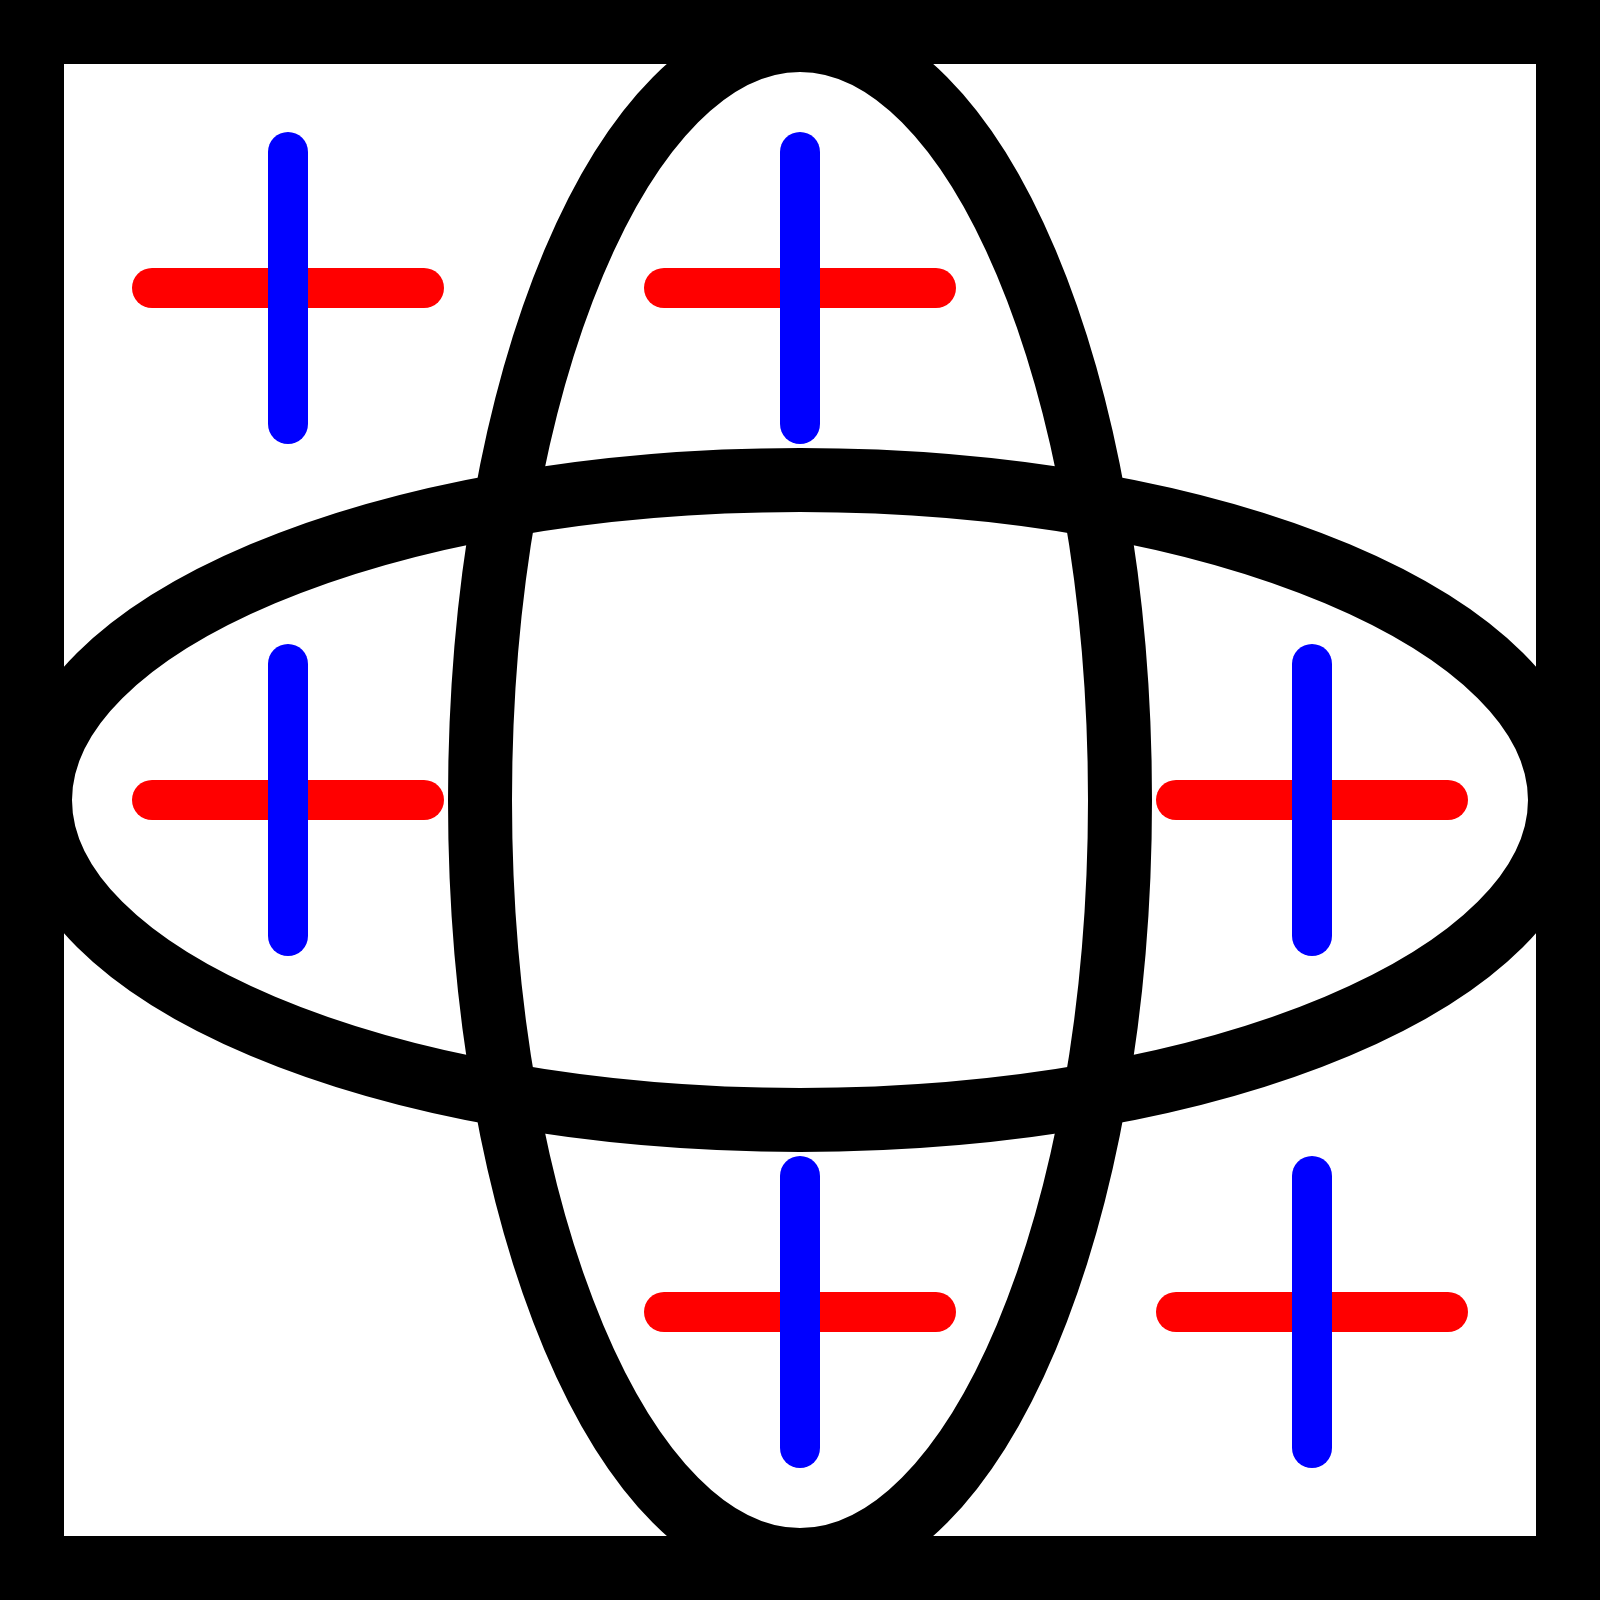
\includegraphics[width=300px]{img/empty-diagonal.png}
    \caption{Hra po devíti tazích optimální strategie}
    \label{fig:empty-diagonal}
\end{figure}

Ať zahraje první hráč kamkoli, druhý hráč bude hrát na další volné políčko v
diagonále. První hráč následně zabere třetí volné políčko (jedno už zabral on,
na druhé hrát nemůže, protože ho zabral protihráč v právě předchozím tahu).
Druhému hráč už tak pouze zbývá jedno jediné políčko, na které může hrát, které
ho dovede k vítězství, viz obrázek \ref{fig:last-diagonal}.

\begin{figure}[h]
    \centering
    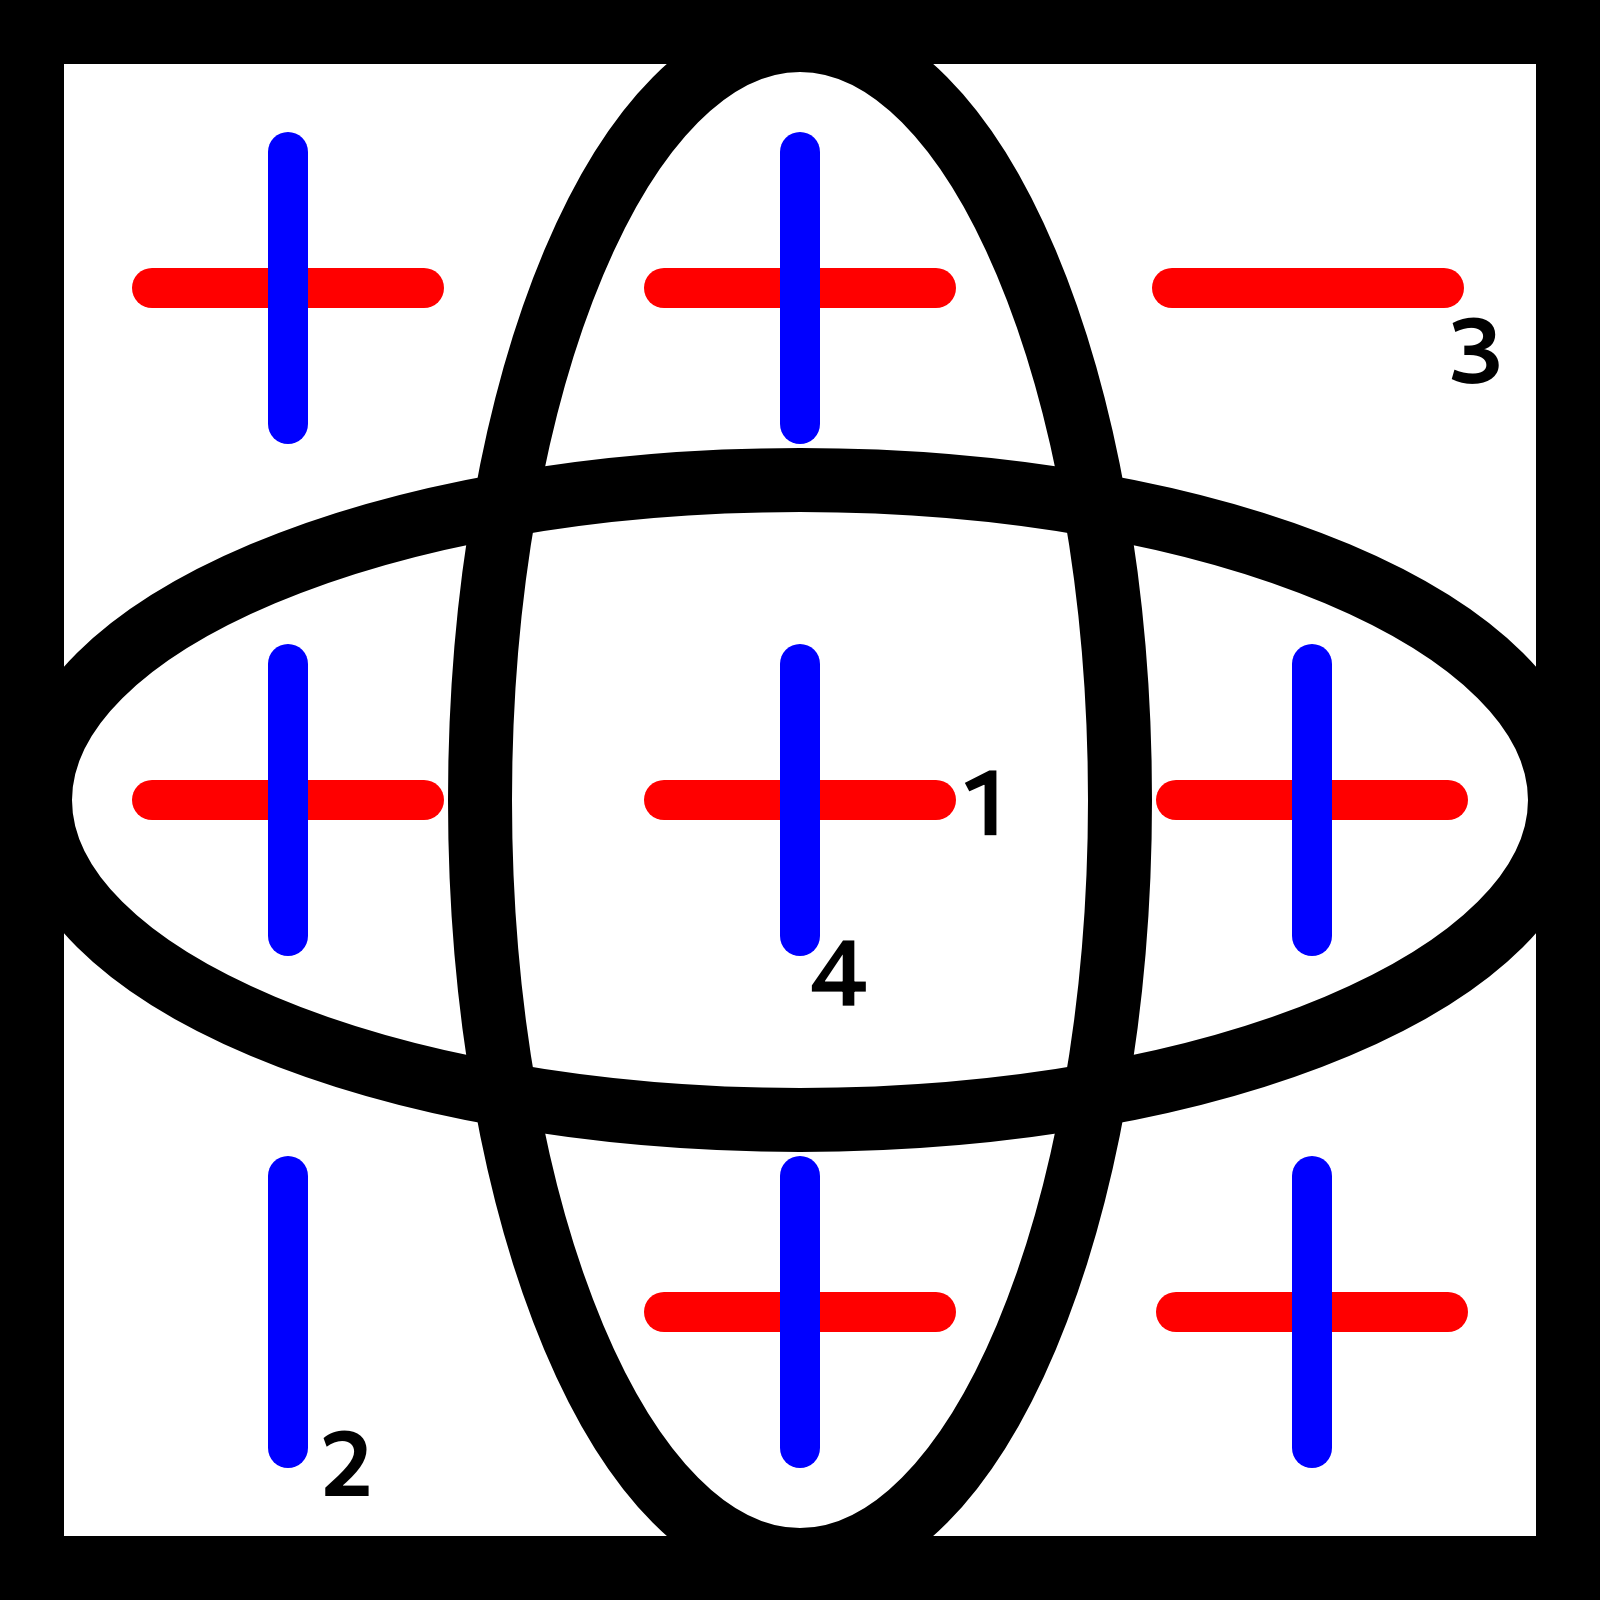
\includegraphics[width=300px]{img/last-diagonal.png}
    \caption{Možný průběh optimální hry pro poslední diagonálu, tahy očíslované}
    \label{fig:last-diagonal}
\end{figure}
